\documentclass{beamer}

\usepackage[utf8]{inputenc}
\usepackage[spanish]{babel}
\usepackage[T1]{fontenc}
\usepackage{graphicx}
\usepackage{tikz}

% \usepackage{pgfpages}
% \pgfpagesuselayout{2 on 1}[a4paper,border shrink=5mm]


\renewcommand\shorthandsspanish{}
\noextrasspanish

\title{Python como Entorno Científico de Desarrollo}
\author{
Guillem Borrell i Nogueras\\
\texttt{guillemborrell@gmail.com}
}

\begin{document}

\begin{frame}
\begin{center}
 
\includegraphics[width=9cm]{files/python-logo-generic.pdf}\\
 % python-logo-generic.pdf: 389x115 pixel, 72dpi, 13.72x4.06 cm, bb=0 0 389 115
\begin{large}
\textbf{Python como Entorno de Desarrollo Científico}
\end{large}\\

Guillem Borrell i Nogueras\\

Curso i-MATH, Julio-Septiembre de 2008
\end{center}

\end{frame}


\begin{frame}
 \frametitle{Dos mundos distintos}
\begin{center}
 \begin{tabular}[h]{cc}
   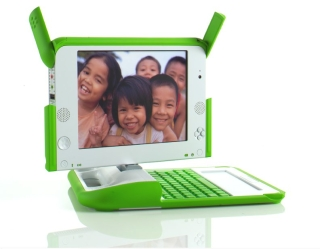
\includegraphics[width=5cm]{files/nigerian-machine.jpg} &
   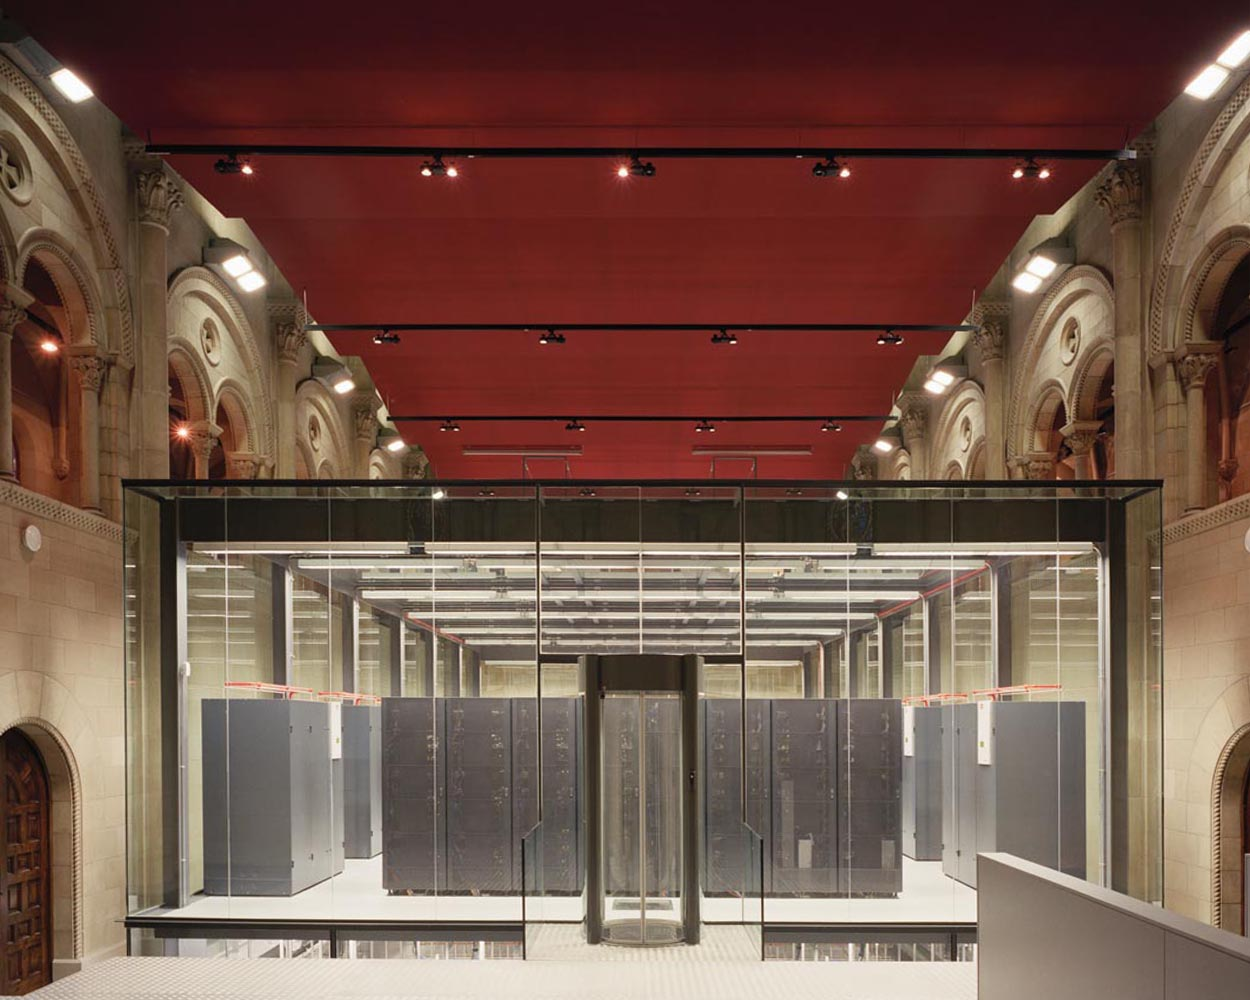
\includegraphics[width=5cm]{files/marenostrum.jpg}\\
   Pequeño & Grande
 \end{tabular}
\end{center}
\end{frame}

\begin{frame}
\frametitle{Scripts}
\begin{itemize}
\item 1 Procesador
\item 1 Thread
\item ejecución $\sim$ segundos
\item GUI
\item Normalmente < $10^3$ lineas de código.
\end{itemize}
\end{frame}

\begin{frame}
\frametitle{HPC}
\begin{itemize}
\item > 8 Procesadores
\item > 8 Procesos o Threads
\item ejecución $\sim$ horas
\item no GUI
\item Quizás > $10^3$ líneas de código.
\end{itemize}
\end{frame}

\begin{frame}
 \frametitle{Dos mundos distintos}
\begin{center}
 \begin{tabular}[h]{cc}
   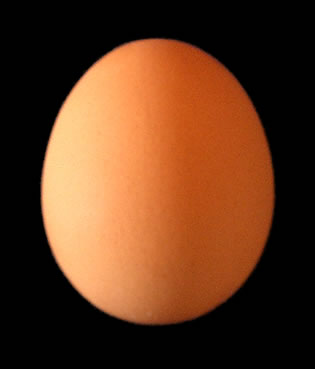
\includegraphics[width=5cm]{files/huevo.jpg} &
   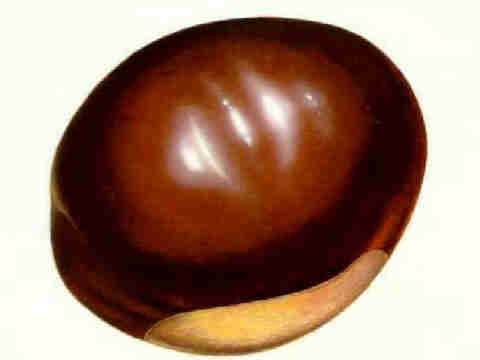
\includegraphics[width=5cm]{files/castana.jpg}\\
   Huevo & Castaña
 \end{tabular}
\end{center}
\end{frame}


\begin{frame}
 \frametitle{¿Por qué se llama Python?}
 Python debe su nombre a...
\end{frame}

\begin{frame}
 \begin{center}
 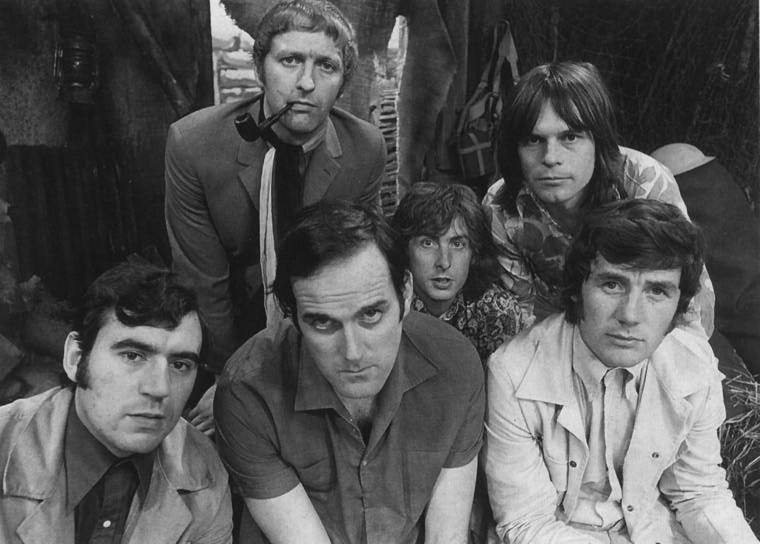
\includegraphics[width=9cm]{files/python.jpg}\\
 % python.jpg: 760x544 pixel, 72dpi, 26.81x19.19 cm, bb=0 0 760 544
Monty Python
\end{center}

\end{frame}

\begin{frame}
 \frametitle{¿Quién usa Python?}

\begin{center}
 
\includegraphics[width=3cm]{files/google.jpg}
 
\includegraphics[width=3cm]{files/Industrial_Light_and_Magic.jpg}
 
\includegraphics[width=3cm]{files/NASA_Logo.jpg}
 
\includegraphics[width=3cm]{files/honeywell_logo.jpg}
\end{center}
\end{frame}

\begin{frame}
 \frametitle{¿Para qué sirve Python?}
 \begin{center}
 Prácticamente para cualquier cosa que se nos pueda ocurrir
 \end{center}

\end{frame}

\begin{frame}
 \frametitle{Desde páginas web...}
\begin{center}
 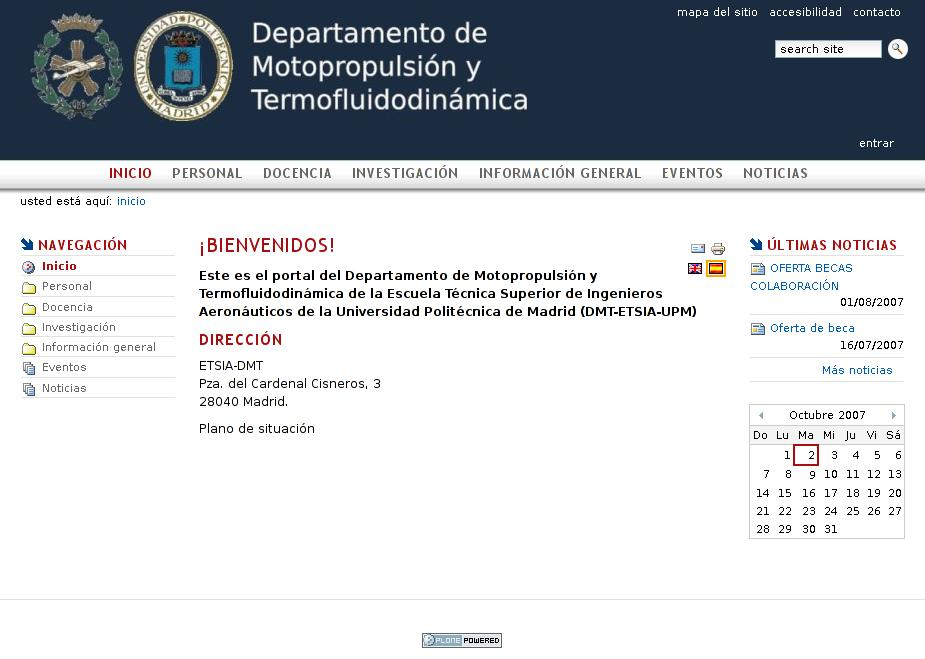
\includegraphics[width=9cm]{files/snapshot1.jpg}\\
 % snapshot1.jpg: 925x659 pixel, 762dpi, 3.08x2.20 cm, bb=0 0 87 62
Plone, Zope
\end{center}

\end{frame}

\begin{frame}
 \frametitle{...A utilidades para bioinformática}
\begin{center}
 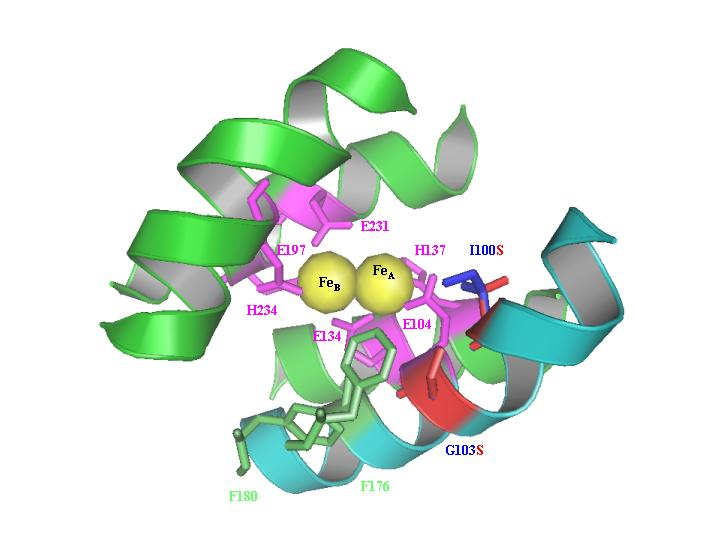
\includegraphics[width=8cm]{files/pymol.jpg}\\
 % pymol.jpg: 720x540 pixel, 72dpi, 25.40x19.05 cm, bb=0 0 720 540
Pymol
\end{center}

\end{frame}

\begin{frame}
 \frametitle{Principales características de Python}

\begin{itemize}
 \item Software Libre (Licencia estilo BSD)
 \item Interpretado
 \item Interactivo
 \item Multiparadigma
 \begin{itemize}
  \item Procedimental
  \item Modular
  \item Orientado a Objetos
 \end{itemize}
 \item Multiplataforma
 \item Especificación especialmente corta (IronPython, Jython, PyPy,
   tinypy ...)
 \item \emph{Incluye las pilas}
 \item ...
\end{itemize}

\end{frame}

\begin{frame}
 \frametitle{¿Por qué Python se está volviendo tan popular}
\begin{itemize}
 \item Fácil de aprender
 \item Fácil de ampliar
 \item Consistente por diseño
 \item Impone un buen estilo de programación
 \item Soporta todas las prácticas propuestas por XP, Agile.
\end{itemize}
\begin{center}
 Porque es divertido
\end{center}
\end{frame}

\begin{frame}
 \frametitle{¿Por qué Python y no otro lenguaje?}
\begin{itemize}
 \item Fácilmente extensible.
 \begin{itemize}
 \item CPython, escrito en ANSI C.
\end{itemize}
 \item Dinámico.
 \item Software Libre.
 \item Excelente documentación.
\end{itemize}

\end{frame}


\begin{frame}
\begin{center}
\begin{LARGE}
¿Qué pinta tiene código escrito en Python?
\end{LARGE} 
\end{center}
\end{frame}

\begin{frame}[containsverbatim]
 \frametitle{Todo es un objeto}
\begin{verbatim}
guillem@aiguaviva ~ $ python
Python 2.4.4 (#1, Sep 25 2007, 21:44:53)
[GCC 4.1.2 (Gentoo 4.1.2)] on linux2
Type "help", "copyright", "credits" or "license" ...
>>> import cmath
>>> i=cmath.sqrt(-1) #Los namespaces son objetos
>>> i.conjugate() #Los números son objetos
-1j
>>> i.imag
1.0
>>> i.real
0.0
>>> i+=3 
>>> i
(3+1j)
\end{verbatim}
\end{frame}

\begin{frame}[containsverbatim]
 \frametitle{Definir funciones es muy fácil}
\begin{verbatim}
>>> def sumauno(numero):
...     return numero+1
...
>>> sumauno(i)
(4+1j)
\end{verbatim}
\begin{itemize}
 \item No hay llaves ni ends, los niveles se definen por el sangrado.
\end{itemize}
\end{frame}

\begin{frame}[containsverbatim]
 \frametitle{Documentación a la Matlab}
\begin{verbatim}
>>> def docfunc():
...     """Esta es una función documentada, a diferencia
...     de Matlab la documentación de las funciones de
...     Python es extraíble y formateable"""
...     pass
...
>>> help(docfunc)
Help on function docfunc in module __main__:

docfunc()
    Esta es una función documentada, a diferencia de
    Matlab la documentación de las funciones de Python
    es extraíble y formateable
\end{verbatim}
\end{frame}


\begin{frame}[containsverbatim]
\frametitle{Una clase llamada pato}
\begin{verbatim}
 >>> class pato:
...     cantidad = 1
...     def haz_cua(self):
...           print "cua!"
...
...     def reproducete(self):
...           cantidad += 1
...
>>> estoesunpato=pato() #instancia de pato
>>> estoesunpato.cantidad
1
>>> estoesunpato.haz_cua()
cua!
\end{verbatim} 
\end{frame}

\begin{frame}[containsverbatim]
 \frametitle{Duck Typing}
Si algo anda como un pato y hace cua como un pato para mi va a ser un pato.
\begin{verbatim}
>>> estoesunpato=pato() #instancia de pato
>>> cuaqueador(estoesunpato)
cua!
>>> class guillem:
...     def haz_cua(self):
...             print "cua!"
...
>>> falsopato=guillem() #ese soy yo
>>> cuaqueador(falsopato)
cua!
>>> isinstance(falsopato,pato)
False
\end{verbatim}
Para la función cuaqueador yo soy tan pato como un pato.
\end{frame}

%%%%%%%%%%%%%%%% Scripting %%%%%%%%%%%%%%%%%%

\begin{frame}
 \frametitle{python para huevos (pequeños)}
  \begin{center}
 \begin{tabular}[h]{ccc}
   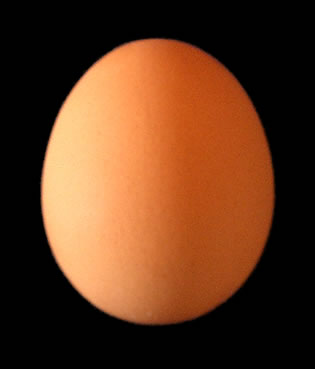
\includegraphics[width=5cm]{files/huevo.jpg} & &
   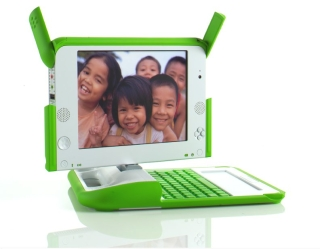
\includegraphics[width=5cm]{files/nigerian-machine.jpg}\\
   Huevo & = &Pequeño
 \end{tabular}
\end{center}
\end{frame}

\begin{frame}
  \frametitle{Somos insaciables.}
Queremos un lenguaje de programación...
  \begin{itemize}
  \item Que sea completo según Turing.
  \item Que lo haga \textbf{todo}
  \item Que lo haga \textbf{bien}
  \item Que no me cueste
  \item Que no tenga que mirar el manual
  \item Que ejecute en cualquier sitio.
  \end{itemize}
\end{frame}

\begin{frame}
  \frametitle{¿Java?}
  \begin{itemize}
  \item ¿Matemáticas con Java?
  \item ¿Ganancia respecto a C++?
  \item ¿Existe una comunidad de usuarios?
  \end{itemize}
\end{frame}

\begin{frame}
  \frametitle{Matlab}
  \begin{itemize}
  \item Uno de los lenguajes de programación más patéticos que he
    visto
  \item ¿Por qué pagar $\sim$ 10000 Euros por algo que no lo vale?
  \end{itemize}
\end{frame}

\begin{frame}
  \frametitle{Mathematica, Maple...}
  \begin{center}
    DSL. He dicho lenguaje de programación.
  \end{center}
\end{frame}

%%%%%%%%%%%%%%%% HPC %%%%%%%%%%%%%%%%%%


\begin{frame}
 \frametitle{python para castañas (grandes)}
  \begin{center}
 \begin{tabular}[h]{ccc}
   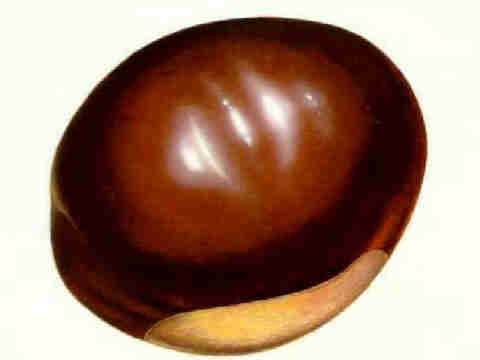
\includegraphics[width=5cm]{files/castana.jpg}& &
   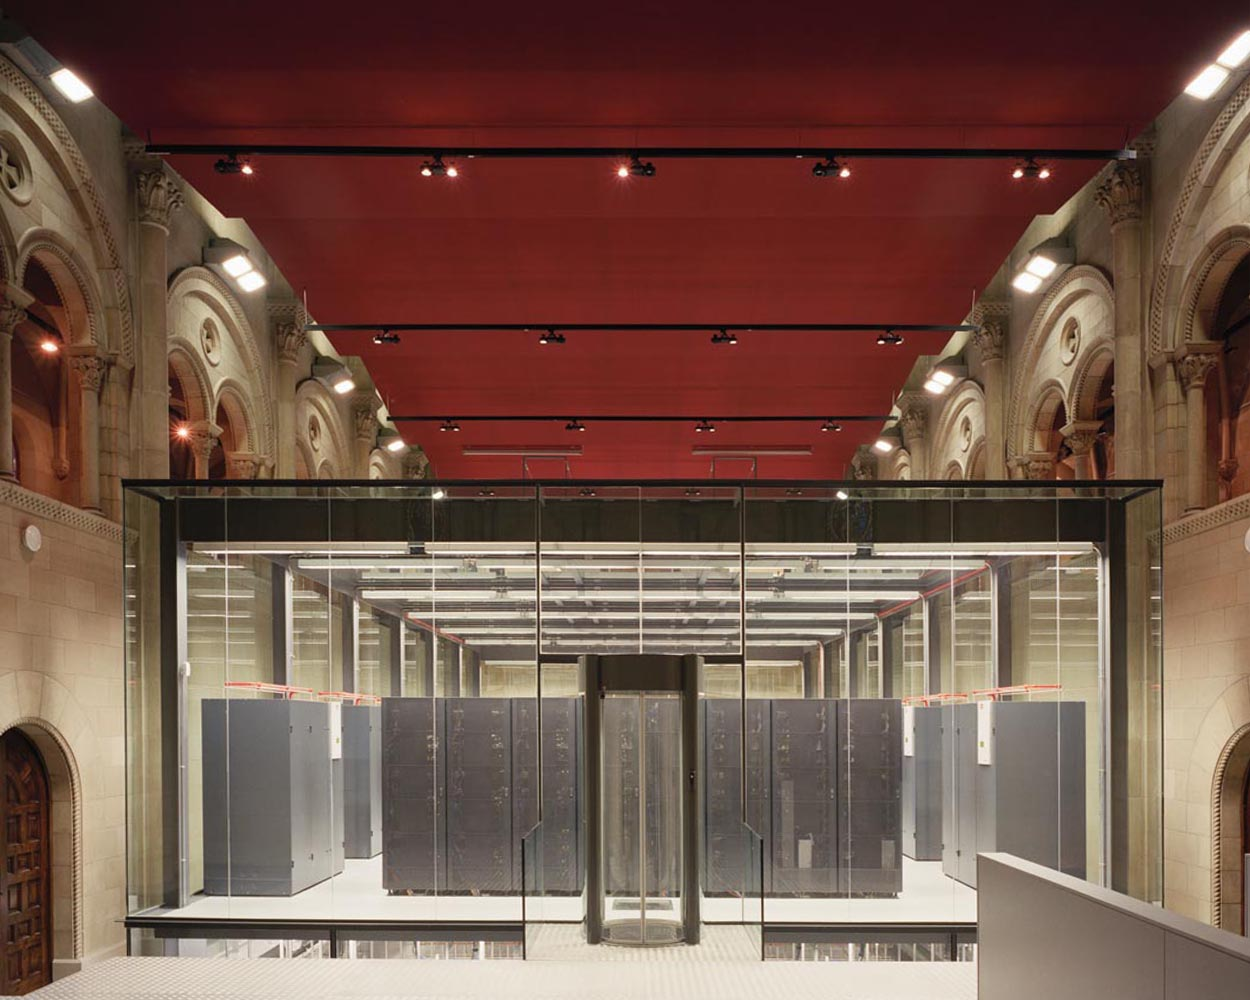
\includegraphics[width=5cm]{files/marenostrum.jpg}\\
   Castaña & = & Grande
 \end{tabular}
\end{center}
\end{frame}

\begin{frame}
  \frametitle{Same old story}
  \begin{center}
    \begin{Huge}
      \textbf{HPC = Fortran, C}
    \end{Huge}
  \end{center}
\end{frame}

\begin{frame}[containsverbatim]
 \frametitle{Arrays}
El objetivo es encajar
\begin{verbatim}
 double array[ ];
\end{verbatim}
en:
\begin{verbatim}
typedef struct PyArrayObject { 
    PyObject HEAD
    char * data;
    int nd;
    intp * dimensions;
    intp * strides;
    PyObject * base;
    PyArray Descr * descr;
    int flags;
    PyObject * weakreflist;
};
\end{verbatim}
\end{frame}

\begin{frame}
 \frametitle{Posibles problemas}
\begin{itemize}
 \item Hacerlo manualmente requiere C medio
 \item Conocimiento del intérprete
 \item Problemas de alineación (strides)
 \item ¿Como Fortran o como C?
\end{itemize}
\begin{center}
 ¿No era tan fácil?
\end{center}
\end{frame}

\begin{frame}
 \frametitle{Es fácil gracias a...}
\begin{itemize}
 \item ctypes
 \item f2py
\end{itemize}

\end{frame}

\begin{frame}
 \frametitle{ctypes}
Permite enlazar en tiempo de ejecución una librería al intérprete
\end{frame}

\begin{frame}[containsverbatim]
 \frametitle{Un wrapper inútil.}
\begin{verbatim}
from ctypes import c_int, POINTER #1
import numpy as np
from numpy.ctypeslib import load_library,ndpointer #1

def dgesv(N,A,B):
    A = np.asfortranarray(A.astype(np.float64)) #2
    B = np.asfortranarray(B.astype(np.float64))

    cN=c_int(N)
    NRHS=c_int(1)
    LDA=c_int(N)
    IPIV=(c_int * N)()
    LDB=c_int(N)
    INFO=c_int(1)

    lapack=load_library('liblapack.so','/usr/lib/')#3
...
\end{verbatim}
\end{frame}

\begin{frame}[containsverbatim]
 \begin{verbatim}
     lapack.dgesv_.argtypes=[POINTER(c_int),
             POINTER(c_int),
             ndpointer(dtype=np.float64,
             ndim=2,
             flags='FORTRAN'),
             POINTER(c_int), POINTER(c_int),
             ndpointer(dtype=np.float64,
                       ndim=2,
                       flags='FORTRAN'),
             POINTER(c_int),POINTER(c_int)]#4

    lapack.dgesv_(cN,NRHS,A,LDA,IPIV,B,LDB,INFO)#5
    return B

print dgesv(2,np.array([[1,2],[1,4]]),np.array([[1,3]]))
\end{verbatim}
\end{frame}

\begin{frame}
 \begin{center}
  \begin{huge}
   ¡No hay que programar en C!
  \end{huge}
 \end{center}
\vspace{2cm}
\begin{itemize}
 \item FORTRAN (trailing underscore)
 \item Conversión de arrays
 \item Llamadas por referencia
 \item Toda subrutina puede ser una librería, sólo hay que compilarla de otra manera.
 \item Velocidad de ejecución $\sim$ Fortran
 \item Reciclaje
\end{itemize}
\end{frame}

\begin{frame}
 \frametitle{f2py}
Es una aplicación que es capaz de entender la mayoría del código en Fortran y lo convierte automáticamente en un módulo de Python
\end{frame}


\begin{frame}[containsverbatim]
 \frametitle{Aún más fácil con f2py}
\begin{verbatim}
!t.f90
subroutine withCallback(a, b, ipar, rpar, callback)
  real a,b, rpar(*)
  integer ipar(*)
  external callback
  print*, 'The parameters are', a,b, ipar(:3), rpar(:3)
  call callback(rpar, ipar)
end subroutine withCallback

subroutine theCallback(rpar, ipar)
  real rpar(*)
  integer ipar(*)
  print*, 'Here the callback is called', ipar(:3), rpar(:3)
end subroutine theCallback
\end{verbatim}
\end{frame}

\begin{frame}[containsverbatim]
 \frametitle{Y funciona...}
\begin{verbatim}
$ f2py -c -m callback t.f90 --fcompiler=gnu95

>>> from numpy import *
>>> import callback
>>> ipar=array([4,5,6])
>>> rpar=array([1.,2.,3.])
>>> callback.withcallback(8,9,ipar,rpar,
...    callback.thecallback)
 The parameters are   8.000000       9.000000    4      5 
         6   1.000000       2.000000       3.000000
 Here the callback is called           4       5     6  
1.000000       2.000000       3.000000
>>>
\end{verbatim}
\end{frame}

\begin{frame}
 \begin{center}
 \begin{huge}
  Ahora sí parece más fácil.
 \end{huge}
\end{center}
\end{frame}

\begin{frame}
 \frametitle{Python en paralelo}
\begin{center}
% Graphic for TeX using PGF
% Title: /home/guillem/CursoScripting/clases/slides/seminario_python_escuela_oct2007/files/diagrama_par.dia
% Creator: Dia v0.95-1
% CreationDate: Wed Oct 10 15:09:50 2007
% For: guillem
% \usepackage{tikz}
% The following commands are not supported in PSTricks at present
% We define them conditionally, so when they are implemented,
% this pgf file will use them.
\ifx\du\undefined
  \newlength{\du}
\fi
\setlength{\du}{15\unitlength}
\begin{tikzpicture}
\pgftransformxscale{1.000000}
\pgftransformyscale{-1.000000}
\definecolor{dialinecolor}{rgb}{0.000000, 0.000000, 0.000000}
\pgfsetstrokecolor{dialinecolor}
\definecolor{dialinecolor}{rgb}{1.000000, 1.000000, 1.000000}
\pgfsetfillcolor{dialinecolor}
\definecolor{dialinecolor}{rgb}{1.000000, 1.000000, 1.000000}
\pgfsetfillcolor{dialinecolor}
\fill (19.100000\du,7.000000\du)--(19.100000\du,8.900000\du)--(22.200000\du,8.900000\du)--(22.200000\du,7.000000\du)--cycle;
\pgfsetlinewidth{0.100000\du}
\pgfsetdash{}{0pt}
\pgfsetdash{}{0pt}
\pgfsetmiterjoin
\definecolor{dialinecolor}{rgb}{0.000000, 0.000000, 0.000000}
\pgfsetstrokecolor{dialinecolor}
\draw (19.100000\du,7.000000\du)--(19.100000\du,8.900000\du)--(22.200000\du,8.900000\du)--(22.200000\du,7.000000\du)--cycle;
% setfont left to latex
\definecolor{dialinecolor}{rgb}{0.000000, 0.000000, 0.000000}
\pgfsetstrokecolor{dialinecolor}
\node at (20.650000\du,8.100000\du){mpirun};
\definecolor{dialinecolor}{rgb}{1.000000, 1.000000, 1.000000}
\pgfsetfillcolor{dialinecolor}
\fill (10.000000\du,11.000000\du)--(10.000000\du,16.000000\du)--(17.000000\du,16.000000\du)--(17.000000\du,11.000000\du)--cycle;
\pgfsetlinewidth{0.100000\du}
\pgfsetdash{}{0pt}
\pgfsetdash{}{0pt}
\pgfsetmiterjoin
\definecolor{dialinecolor}{rgb}{0.000000, 0.000000, 0.000000}
\pgfsetstrokecolor{dialinecolor}
\draw (10.000000\du,11.000000\du)--(10.000000\du,16.000000\du)--(17.000000\du,16.000000\du)--(17.000000\du,11.000000\du)--cycle;
% setfont left to latex
\definecolor{dialinecolor}{rgb}{0.000000, 0.000000, 0.000000}
\pgfsetstrokecolor{dialinecolor}
\node[anchor=west] at (10.450000\du,13.650000\du){Proceso};
\definecolor{dialinecolor}{rgb}{1.000000, 1.000000, 1.000000}
\pgfsetfillcolor{dialinecolor}
\fill (13.500000\du,12.000000\du)--(13.500000\du,15.000000\du)--(16.600000\du,15.000000\du)--(16.600000\du,12.000000\du)--cycle;
\pgfsetlinewidth{0.100000\du}
\pgfsetdash{}{0pt}
\pgfsetdash{}{0pt}
\pgfsetmiterjoin
\definecolor{dialinecolor}{rgb}{0.000000, 0.000000, 0.000000}
\pgfsetstrokecolor{dialinecolor}
\draw (13.500000\du,12.000000\du)--(13.500000\du,15.000000\du)--(16.600000\du,15.000000\du)--(16.600000\du,12.000000\du)--cycle;
% setfont left to latex
\definecolor{dialinecolor}{rgb}{0.000000, 0.000000, 0.000000}
\pgfsetstrokecolor{dialinecolor}
\node at (15.050000\du,13.650000\du){Python};
% setfont left to latex
\definecolor{dialinecolor}{rgb}{0.000000, 0.000000, 0.000000}
\pgfsetstrokecolor{dialinecolor}
\node[anchor=west] at (12.000000\du,10.000000\du){CPU 0};
\definecolor{dialinecolor}{rgb}{1.000000, 1.000000, 1.000000}
\pgfsetfillcolor{dialinecolor}
\fill (17.400000\du,10.950000\du)--(17.400000\du,15.950000\du)--(24.400000\du,15.950000\du)--(24.400000\du,10.950000\du)--cycle;
\pgfsetlinewidth{0.100000\du}
\pgfsetdash{}{0pt}
\pgfsetdash{}{0pt}
\pgfsetmiterjoin
\definecolor{dialinecolor}{rgb}{0.000000, 0.000000, 0.000000}
\pgfsetstrokecolor{dialinecolor}
\draw (17.400000\du,10.950000\du)--(17.400000\du,15.950000\du)--(24.400000\du,15.950000\du)--(24.400000\du,10.950000\du)--cycle;
% setfont left to latex
\definecolor{dialinecolor}{rgb}{0.000000, 0.000000, 0.000000}
\pgfsetstrokecolor{dialinecolor}
\node[anchor=west] at (17.850000\du,13.600000\du){Proceso};
\definecolor{dialinecolor}{rgb}{1.000000, 1.000000, 1.000000}
\pgfsetfillcolor{dialinecolor}
\fill (21.050000\du,11.900000\du)--(21.050000\du,14.900000\du)--(24.150000\du,14.900000\du)--(24.150000\du,11.900000\du)--cycle;
\pgfsetlinewidth{0.100000\du}
\pgfsetdash{}{0pt}
\pgfsetdash{}{0pt}
\pgfsetmiterjoin
\definecolor{dialinecolor}{rgb}{0.000000, 0.000000, 0.000000}
\pgfsetstrokecolor{dialinecolor}
\draw (21.050000\du,11.900000\du)--(21.050000\du,14.900000\du)--(24.150000\du,14.900000\du)--(24.150000\du,11.900000\du)--cycle;
% setfont left to latex
\definecolor{dialinecolor}{rgb}{0.000000, 0.000000, 0.000000}
\pgfsetstrokecolor{dialinecolor}
\node at (22.600000\du,13.550000\du){Python};
% setfont left to latex
\definecolor{dialinecolor}{rgb}{0.000000, 0.000000, 0.000000}
\pgfsetstrokecolor{dialinecolor}
\node[anchor=west] at (21.000000\du,10.000000\du){CPU 1};
\definecolor{dialinecolor}{rgb}{1.000000, 1.000000, 1.000000}
\pgfsetfillcolor{dialinecolor}
\fill (24.750000\du,10.900000\du)--(24.750000\du,15.900000\du)--(31.750000\du,15.900000\du)--(31.750000\du,10.900000\du)--cycle;
\pgfsetlinewidth{0.100000\du}
\pgfsetdash{}{0pt}
\pgfsetdash{}{0pt}
\pgfsetmiterjoin
\definecolor{dialinecolor}{rgb}{0.000000, 0.000000, 0.000000}
\pgfsetstrokecolor{dialinecolor}
\draw (24.750000\du,10.900000\du)--(24.750000\du,15.900000\du)--(31.750000\du,15.900000\du)--(31.750000\du,10.900000\du)--cycle;
% setfont left to latex
\definecolor{dialinecolor}{rgb}{0.000000, 0.000000, 0.000000}
\pgfsetstrokecolor{dialinecolor}
\node[anchor=west] at (25.200000\du,13.550000\du){Proceso};
\definecolor{dialinecolor}{rgb}{1.000000, 1.000000, 1.000000}
\pgfsetfillcolor{dialinecolor}
\fill (28.350000\du,11.750000\du)--(28.350000\du,14.750000\du)--(31.450000\du,14.750000\du)--(31.450000\du,11.750000\du)--cycle;
\pgfsetlinewidth{0.100000\du}
\pgfsetdash{}{0pt}
\pgfsetdash{}{0pt}
\pgfsetmiterjoin
\definecolor{dialinecolor}{rgb}{0.000000, 0.000000, 0.000000}
\pgfsetstrokecolor{dialinecolor}
\draw (28.350000\du,11.750000\du)--(28.350000\du,14.750000\du)--(31.450000\du,14.750000\du)--(31.450000\du,11.750000\du)--cycle;
% setfont left to latex
\definecolor{dialinecolor}{rgb}{0.000000, 0.000000, 0.000000}
\pgfsetstrokecolor{dialinecolor}
\node at (29.900000\du,13.400000\du){Python};
% setfont left to latex
\definecolor{dialinecolor}{rgb}{0.000000, 0.000000, 0.000000}
\pgfsetstrokecolor{dialinecolor}
\node[anchor=west] at (28.300000\du,10.000000\du){CPU n};
\pgfsetlinewidth{0.100000\du}
\pgfsetdash{}{0pt}
\pgfsetdash{}{0pt}
\pgfsetmiterjoin
\pgfsetbuttcap
{
\definecolor{dialinecolor}{rgb}{0.000000, 0.000000, 0.000000}
\pgfsetfillcolor{dialinecolor}
% was here!!!
\pgfsetarrowsend{stealth}
{\pgfsetcornersarced{\pgfpoint{0.000000\du}{0.000000\du}}\definecolor{dialinecolor}{rgb}{0.000000, 0.000000, 0.000000}
\pgfsetstrokecolor{dialinecolor}
\draw (20.650000\du,8.900000\du)--(20.650000\du,10.450000\du)--(15.050000\du,10.450000\du)--(15.050000\du,12.000000\du);
}}
\pgfsetlinewidth{0.100000\du}
\pgfsetdash{}{0pt}
\pgfsetdash{}{0pt}
\pgfsetmiterjoin
\pgfsetbuttcap
{
\definecolor{dialinecolor}{rgb}{0.000000, 0.000000, 0.000000}
\pgfsetfillcolor{dialinecolor}
% was here!!!
\pgfsetarrowsend{stealth}
{\pgfsetcornersarced{\pgfpoint{0.000000\du}{0.000000\du}}\definecolor{dialinecolor}{rgb}{0.000000, 0.000000, 0.000000}
\pgfsetstrokecolor{dialinecolor}
\draw (20.650000\du,8.900000\du)--(20.650000\du,10.450010\du)--(22.600000\du,10.450010\du)--(22.600000\du,11.900000\du);
}}
\pgfsetlinewidth{0.100000\du}
\pgfsetdash{}{0pt}
\pgfsetdash{}{0pt}
\pgfsetmiterjoin
\pgfsetbuttcap
{
\definecolor{dialinecolor}{rgb}{0.000000, 0.000000, 0.000000}
\pgfsetfillcolor{dialinecolor}
% was here!!!
\pgfsetarrowsend{stealth}
{\pgfsetcornersarced{\pgfpoint{0.000000\du}{0.000000\du}}\definecolor{dialinecolor}{rgb}{0.000000, 0.000000, 0.000000}
\pgfsetstrokecolor{dialinecolor}
\draw (20.650000\du,8.900000\du)--(20.650000\du,10.325000\du)--(29.900000\du,10.325000\du)--(29.900000\du,11.750000\du);
}}
\definecolor{dialinecolor}{rgb}{1.000000, 1.000000, 1.000000}
\pgfsetfillcolor{dialinecolor}
\fill (19.450000\du,17.000000\du)--(19.450000\du,19.000000\du)--(24.450000\du,19.000000\du)--(24.450000\du,17.000000\du)--cycle;
\pgfsetlinewidth{0.100000\du}
\pgfsetdash{}{0pt}
\pgfsetdash{}{0pt}
\pgfsetmiterjoin
\definecolor{dialinecolor}{rgb}{0.000000, 0.000000, 0.000000}
\pgfsetstrokecolor{dialinecolor}
\draw (19.450000\du,17.000000\du)--(19.450000\du,19.000000\du)--(24.450000\du,19.000000\du)--(24.450000\du,17.000000\du)--cycle;
% setfont left to latex
\definecolor{dialinecolor}{rgb}{0.000000, 0.000000, 0.000000}
\pgfsetstrokecolor{dialinecolor}
\node at (21.950000\du,18.150000\du){MPI};
\pgfsetlinewidth{0.100000\du}
\pgfsetdash{}{0pt}
\pgfsetdash{}{0pt}
\pgfsetmiterjoin
\pgfsetbuttcap
{
\definecolor{dialinecolor}{rgb}{0.000000, 0.000000, 0.000000}
\pgfsetfillcolor{dialinecolor}
% was here!!!
{\pgfsetcornersarced{\pgfpoint{0.000000\du}{0.000000\du}}\definecolor{dialinecolor}{rgb}{0.000000, 0.000000, 0.000000}
\pgfsetstrokecolor{dialinecolor}
\draw (15.050000\du,15.000000\du)--(15.050000\du,18.000000\du)--(19.450000\du,18.000000\du);
}}
\pgfsetlinewidth{0.100000\du}
\pgfsetdash{}{0pt}
\pgfsetdash{}{0pt}
\pgfsetmiterjoin
\pgfsetbuttcap
{
\definecolor{dialinecolor}{rgb}{0.000000, 0.000000, 0.000000}
\pgfsetfillcolor{dialinecolor}
% was here!!!
{\pgfsetcornersarced{\pgfpoint{0.000000\du}{0.000000\du}}\definecolor{dialinecolor}{rgb}{0.000000, 0.000000, 0.000000}
\pgfsetstrokecolor{dialinecolor}
\draw (22.600000\du,14.900000\du)--(22.600000\du,16.500010\du)--(21.950000\du,16.500010\du)--(21.950000\du,17.000000\du);
}}
\pgfsetlinewidth{0.100000\du}
\pgfsetdash{}{0pt}
\pgfsetdash{}{0pt}
\pgfsetmiterjoin
\pgfsetbuttcap
{
\definecolor{dialinecolor}{rgb}{0.000000, 0.000000, 0.000000}
\pgfsetfillcolor{dialinecolor}
% was here!!!
{\pgfsetcornersarced{\pgfpoint{0.000000\du}{0.000000\du}}\definecolor{dialinecolor}{rgb}{0.000000, 0.000000, 0.000000}
\pgfsetstrokecolor{dialinecolor}
\draw (24.450000\du,18.000000\du)--(29.900000\du,18.000000\du)--(29.900000\du,14.750000\du);
}}
\end{tikzpicture}

\end{center}

\end{frame}

\begin{frame}
 \frametitle{Python en paralelo II}
\begin{itemize}
 \item Se lanza Python como proceso
 \item La comunicación entre los intérpretes puede hacerse mediante MPI
 \begin{itemize}
  \item No hay wrappers para \textbf{blacs} pero pueden hacerse
 \end{itemize}
\end{itemize}
Por ejemplo:
\end{frame}

\begin{frame}
 \frametitle{GIL}
\begin{itemize}
 \item Cpython no es thread safe
 \item No aprovecha los multiple core
 \item Programación concurrente (Threading)
 \begin{itemize}
 \item No hay ganancia respecto a C
 \item ¿Esperar a stackless o pypy?
\end{itemize}
 \item Lo más seguro sigue siendo usar procesos
\end{itemize}
\end{frame}


\end{document}
